\chapter{Diseño del sistema}
%Toda la documentación del sistema hay varias cosas que pueden ir aqui
%
%\begin{itemize}
%    \item Arquitectura del sistema
%    \item Diagrama de clases
%    \item Base de datos
%    \item Diagrama de paquetes
%    \item Diagrama de procesos
%    \item Casos de uso
%    \item Interfaces
%    \item Diseño de la arquitectura de la red neuronal
%\end{itemize}
%No se si tengamos que hacer todos pero al menos la arquitectura del sistema, de la red, casos de uso, interfaces y base de datos yo diría que sí



\section{Arquitectura del sistema}
\begin{figure}[h]
    \centering
    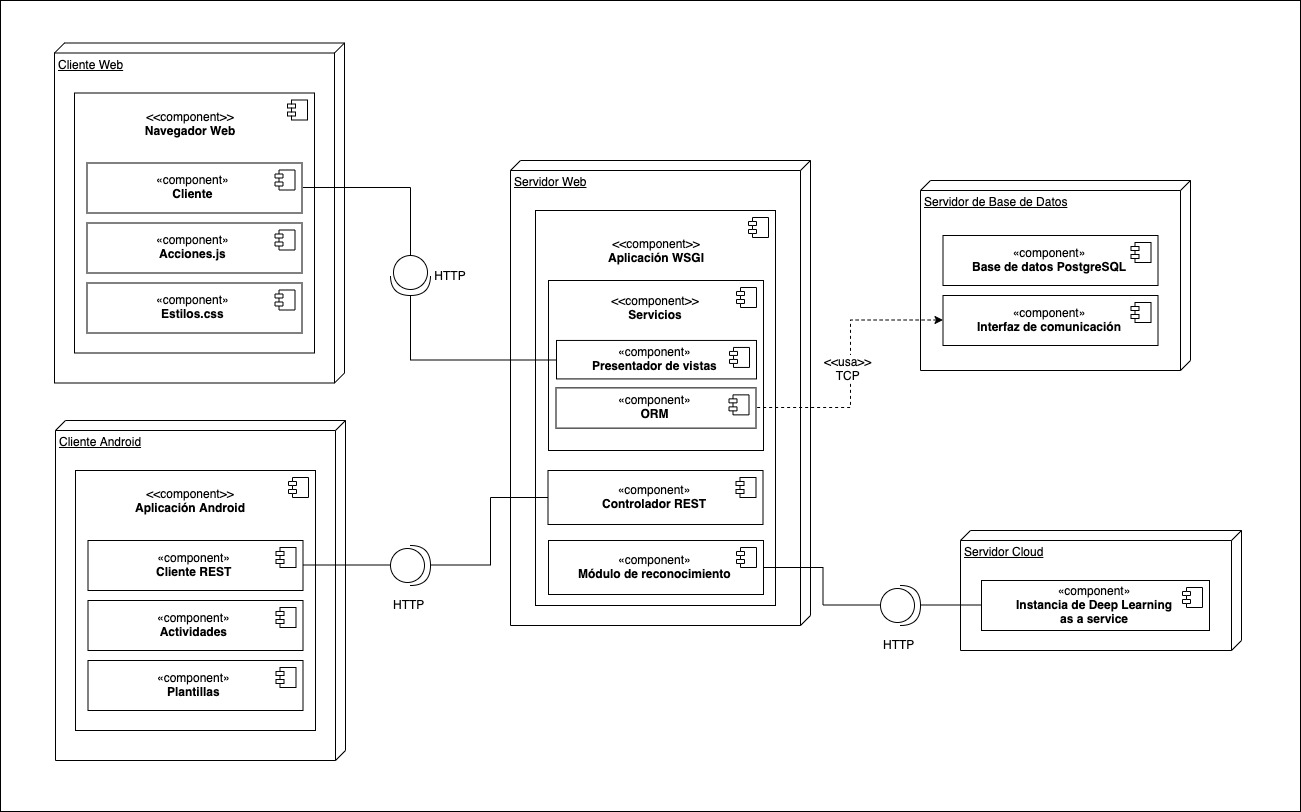
\includegraphics[width=\textwidth]{capitulo4/imagenes/ArquitecturaApp.jpg}
    \caption{Arquitectura del sistema.}
    \label{fig:arquitectura}
\end{figure}

\section{Modelo de datos del sistema}
En la figura \ref{fig:db} se aprecia el modelo de datos del sistema y se describen las entidades que lo conforman, así como los respectivos atributos de cada una de estas entidades.
\begin{figure}[h]
	\centering
	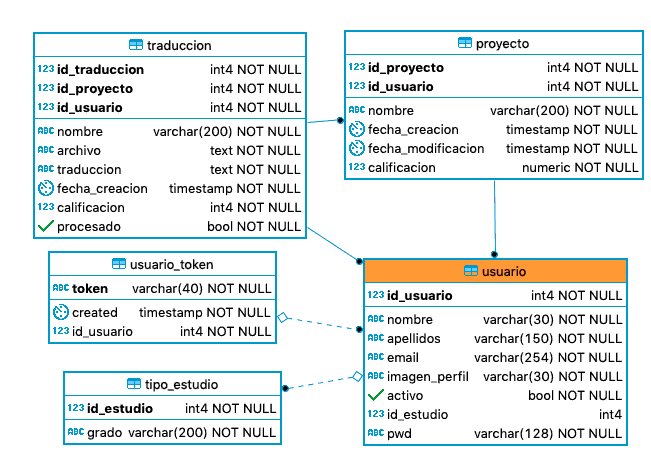
\includegraphics[width=\textwidth]{capitulo4/imagenes/tt_base.png}
	\caption{Modelo de datos del sistema.}
	\label{fig:db}
\end{figure}

\subsection{Entidad: Usuario}
Se refiere a la cuenta que un usuario puede tener, es la forma en la que accede al sistema.
\subsubsection{Atributos}
\begin{center}
	\begin{longtable}{|J{3cm}|J{4cm}|J{3cm}|J{2cm}|J{2cm}|}
		\hline
		\textbf{Nombre} & \textbf{Descripción} & \textbf{Tipo} & \textbf{Requerido} & \textbf{Único} \\ \hline
		id & Llave primaria autoincrementable del usuario & integer & Sí & Sí\\ \hline
		nombre & Nombre que tiene un usuario & varchar(30) & Sí & No \\ \hline
		apellidos & Apellidos de un usuario & varchar(150) & Sí & No \\ \hline
		email & Correo electrónico asociado a un usuario & varchar(254) & Sí & Sí\\ \hline
		imagen\_perfil & Ruta relativa de la ubicación de la imagen de perfil del usuario & varchar(30) & Sí & No \\ \hline
		activo & Bandera que nos permite saber si un usuario ha verificado su cuenta & boolean & Sí & No \\ \hline
		id\_estudios & Identificador para relacionar al usuario con el grado de estudio que tiene del catalogo de tipos de estudios & integer & No & No \\ \hline
		password & Contraseña cifrada del usuario & varchar(128) & Sí & No \\ \hline
		\caption{Tabla de los atributos de la entidad usuario}
		\label{tbl:entidad-usuario}
	\end{longtable}
\end{center}
\subsection{Entidad: Proyecto}
Se refiere a los proyectos que están asociados a un usuario, un proyecto esta compuesto por varias traducciones.
\subsubsection{Atributos}
\begin{center}
	\begin{longtable}{|J{3cm}|J{4cm}|J{3cm}|J{2cm}|J{2cm}|}
		\hline
		\textbf{Nombre} & \textbf{Descripción} & \textbf{Tipo} & \textbf{Requerido} & \textbf{Único} \\ \hline
		id & Identificador autoincrementable del proyecto, forma parte de la llave primaria & integer & Sí & Sí \\ \hline
		usuario\_id & Identificador del usuario que tiene el proyecto, forma parte de la llave primaria & integer & Sí & No \\ \hline
		nombre & Nombre del proyecto & varchar(200) & Sí & No \\ \hline
		fechaModificacion & Fecha que se actualiza cada vez que se modifica el proyecto & timestamp & Sí & No \\ \hline
		fechaCreacion & Fecha en la cual se crea el proyecto & timestamp & Sí & No \\ \hline
		calificacion & Calificación que se calcula a través de las calificaciones de las traducciones asociadas con el proyecto, puede contener decimales & numeric & Sí & No \\ \hline
		\caption{Tabla de los atributos de la entidad proyecto}
		\label{tbl:entidad-proyecto}
	\end{longtable}
\end{center}
\subsection{Entidad: Traducción}
Hace referencia a la traducción de \LaTeX que forma parte de un proyecto y que pertenece a un usuario. Esta traducción es el resultado de analizar una imagen.
\subsubsection{Atributos}
\begin{center}
	\begin{longtable}{|J{3cm}|J{4cm}|J{3cm}|J{2cm}|J{2cm}|}
		\hline
		\textbf{Nombre} & \textbf{Descripción} & \textbf{Tipo} & \textbf{Requerido} & \textbf{Único} \\ \hline
		id & Identificador autoincrementable de la traducción, forma parte de la llave primaria & integer & Sí & Sí \\ \hline
		proyecto\_id & Identificador del proyecto al cual pertenece la traducción, forma parte de la llave primaria & integer & Sí & No \\ \hline
		usuario\_id & Identificador del usuario, forma parte de la llave primaria & integer & Sí & No \\ \hline
		nombre & Nombre que se le da a la traducción & varchar(200) & Sí & No \\ \hline
		calificacion & Calificación que se le da a la traducción para retroalimentación del usuario y del sistema & integer & Sí & No\\ \hline
		fechaCreacion & Fecha en la cual se crea la traducción & timestamp & Sí & No \\ \hline
		\caption{Tabla de los atributos de la entidad traducción}
		\label{tbl:entidad-traduccion}
	\end{longtable}
\end{center}
\subsection{Entidad: Tipo estudios}
Hace referencia a los distintos grados de estudios que tiene un usuario.
\subsubsection{Atributos}
\begin{center}
	\begin{longtable}{|J{3cm}|J{4cm}|J{3cm}|J{2cm}|J{2cm}|}
		\hline
		\textbf{Nombre} & \textbf{Descripción} & \textbf{Tipo} & \textbf{Requerido} & \textbf{Único} \\ \hline
		id & Llave primaria autoincrementable & integer & Sí & Sí \\ \hline
		grado & Nombre del grado de estudio & varchar(200) & Sí & No \\ \hline
		\caption{Tabla de los atributos de la entidad tipo de estudios}
		\label{tbl:entidad-tipo-estudios}
	\end{longtable}
\end{center}
\subsection{Entidad: Usuario Token}
Se refiere al token de autenticación que tiene un usuario al momento de crear una cuenta y que su utiliza en la comunicación entre la aplicación web y android.
\subsubsection{Atributos}
\begin{center}
	\begin{longtable}{|J{3cm}|J{4cm}|J{3cm}|J{2cm}|J{2cm}|}
		\hline
		\textbf{Nombre} & \textbf{Descripción} & \textbf{Tipo} & \textbf{Requerido} & \textbf{Único} \\ \hline
		token & Llave primaria y token de autenticación del usuario para la API REST & varchar(40) & Sí &  Sí\\ \hline
		created & Fecha de generación del token & timestamp & Sí & No\\ \hline
		user\_id & Identificador del usuario al que pertenece el token& integer & Sí & No\\ \hline
		\caption{Tabla de los atributos de la entidad usuario token}
		\label{tbl:entidad-usuario-token}
	\end{longtable}
\end{center}

\section{Aplicación de Android}
\section{Android}
Esta sección tiene objetivo presentar las principales características en el desarrollo de la aplicación para Android.
\subsection{Arquitectura de la aplicación}
Para el desarrollo de la aplicación se implemento la arquitectura Clean, la cual como ya se ha mencionado antes se ha mencionado se ha vuelto muy popular en el desarrollo de aplicaciones móviles para android debido a que es una solución que produce sistemas que presentan las siguientes características.

\begin{itemize}
    \item Escalables, por lo que se pueden agregar más funcionalidades de forma sencilla.
    \item Presentan modularidad.
    \item Presentan independencia en cuanto a frameworks, interfaz de usuario y bases de datos.
    \item El proyecto es más fácil de mantener por lo que es más sencillo hacer cambios.
\end{itemize}

Al utilizar esta arquitectura el proyecto queda separado en tres capas como se observa en la figura \ref{fig:capas-arquitectura} con lo cual cada una de ellas tiene su propósito definido.

\begin{figure}[h]
    \centering
    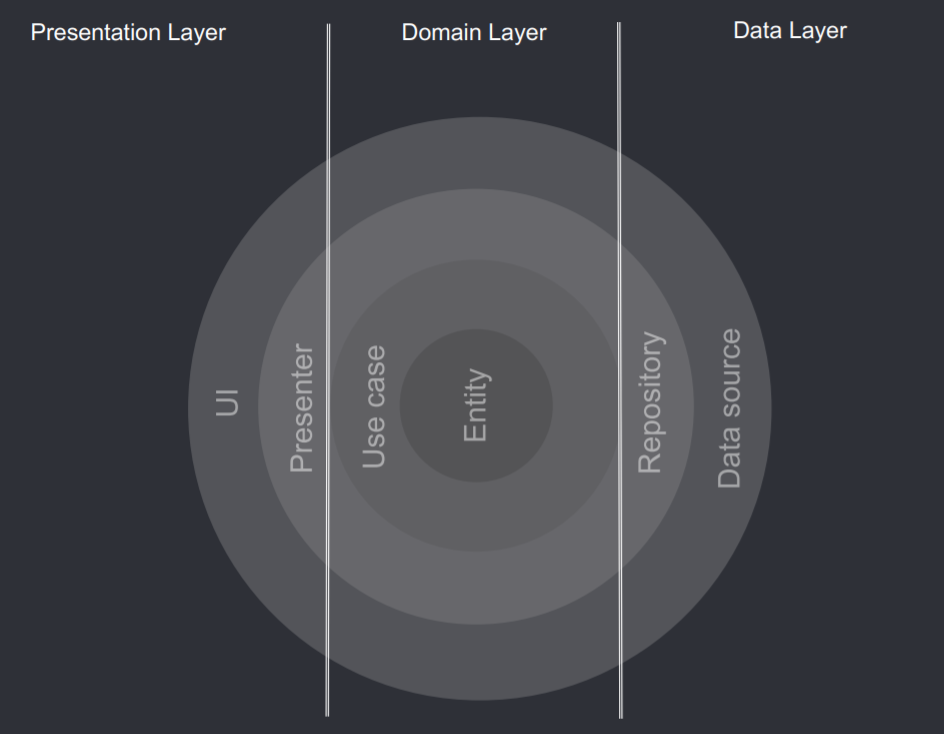
\includegraphics[width=250px]{capitulo5/android/img/capas-clean.png}
    \caption{Tres capas que se tienen al utilizar la arquitectura Clean \cite{cleanGuide}}
    \label{fig:capas-arquitectura}
\end{figure}

\subsubsection{Capa de datos}
La información que se utiliza en el resto de capas proviene de esta capa. Esta capa a su vez se encuentra dividida en la capa de repositorio y en la capa de fuente de datos. 

\paragraph{Capa de repositorio} En esta capa se utiliza el patrón de repositorio como se muestra en la figura \ref{fig:capa-datos}. Gracias a este patrón se puede tener acceso a diferentes fuentes de datos que se encuentran en la capa más baja de nuestra arquitectura, esto nos permite un acceso a los datos de forma transparente para el usuario bajo las condiciones que se presenten.

La forma de utilizar este patrón en la aplicación desarrollado crear una clase en la cual se hace uso de la interfaz que se tiene para el acceso a la fuente de datos. En el siguiente código se puede apreciar el como se crea una instancia de APIService que es nuestra interfaz para fuente de datos.

Después, en nuestro método findAllProyecttosByUser se recupera la información necesaria para mandarla a las capas superiores.

\lstinputlisting[language=Java]{capitulo5/android/src/repositorio.java}

\begin{figure}[h]
    \centering
    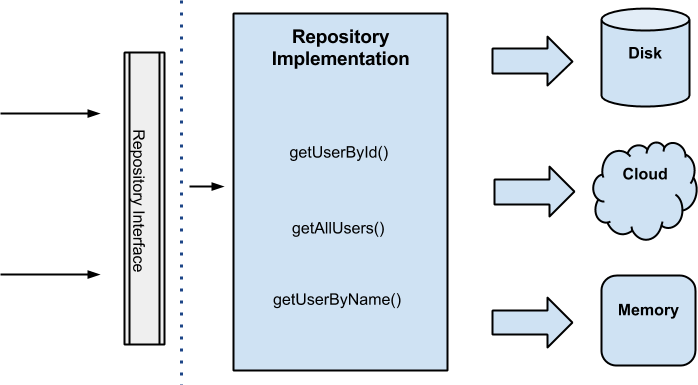
\includegraphics[width=400px]{capitulo5/android/img/capa-datos.png}
    \caption{Capa de datos \cite{cleanWay}}
    \label{fig:capa-datos}
\end{figure}

\paragraph{Capa de fuente de datos} En este trabajo, la fuente de datos que se tiene es un API REST, sin embargo si se requiere acceder a información que se persista en el teléfono se pude agregar otra fuente de datos. Se utilizó retrofit para poder realizar la comunicación con el API REST. 

La forma de utilizar retrofit es crear una interfaz con todos los métodos para recuperar o enviar información al API REST, en esta interfaz cada método tiene la URL a la cual se realizara la petición con alguno de los métodos que tiene HTTP, se tienen los parámetro que se envían y cada método nos regresa una llamada asíncrona que se trabaja en la capa de repositorio. Esto se puede apreciar en el siguiente código.

\lstinputlisting[language=Java]{capitulo5/android/src/APIService.java}

Para poder hacer uso de esta interfaz se tiene que configurar bajo ciertas características especificas como lo son la URL a la cual hará peticiones, el logger que se utilizara para poder observar las peticiones que se realizan y brindar una retroalimentación a la hora de hacer pruebas y por ultimo el parser que se utilizara para trabajar y pasar de clases a datos que el API REST entienda y pueda utilizar, en este caso se utilizo el formato JSON. La definición de estas características se tiene en el siguiente código.

\lstinputlisting[language=Java]{capitulo5/android/src/ServiceGenerator.java}

Finalmente, en esta capa se tienen clases Java que después se mapean a objetos JSON y viceversa, para realizar esto se crea un POJO con los atributos que se necesitan además de agregar anotaciones de retrofit para que el parser pude hacer la conversión necesaria. Un ejemplo de esto es en la siguiente clase de java.

\lstinputlisting[language=Java]{capitulo5/android/src/UsuarioData.java}


\subsubsection{Capa de dominio}
En esta capa es la intermediaria entre las otras dos capas que se tienen, es donde se encuentran los casos de uso también conocidos como interactors como se muestra en la figura \ref{fig:capa-dominio} en ellos la lógica del negocio es ejecutada es por esto que es el núcleo de la aplicación.

Es importante mencionar que esta capa, al ser la encargada del negocio es donde se hacen validaciones en la información y dicha información se adapta para que sea trabajada en la capa de presentación o en la de datos

Además de contener los casos de uso en esta capa se encuentran las entidades y se hace uso de los repositorios para acceder a la información proporcionada por la capa de datos.

\begin{figure}[h]
    \centering
    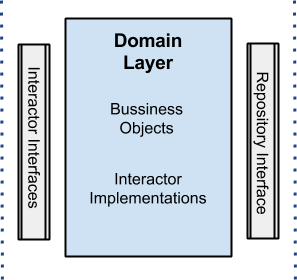
\includegraphics[width=200px]{capitulo5/android/img/capa-dominio.png}
    \caption{Capa de dominio \cite{cleanWay}}
    \label{fig:capa-dominio}
\end{figure}

Para tener un control sobre posibles errores en la capa de presentación o en la capa de datos se utilizan códigos de resultados al igual que una clase que contiene el resultado que se puede presentar, así como la información que se le regresa a la capa de presentación. Se hace uso de genéricos para poder reutilizar esta clase en toda la aplicación y no duplicar código. La clase es la siguiente.

\lstinputlisting[language=Java]{capitulo5/android/src/BusinessResult.java}

La forma en la que se utiliza esta clase en un caso de uso se presenta en el siguiente código que permite iniciar sesión.

\lstinputlisting[language=Java]{capitulo5/android/src/UserInteractorImpl.java}

A su vez el caso de uso utiliza sus propios clases de java para presentar información al usuario en la capa de presentación así como controlar posibles errores en la información que ingrese el usuario los campos de los formularios, un ejemplo de este tipo de clases es el siguiente.

\lstinputlisting[language=Java]{capitulo5/android/src/UsuarioModel.java}

\subsubsection{Capa de presentación}
En esta capa como se muestra en la figura \ref{fig:capa-presentacion} se trabaja con la lógica relacionada a las interfaces que se tienen en la aplicación, es decir a actividades, fragmentos y archivos XML.

\begin{figure}[h]
    \centering
    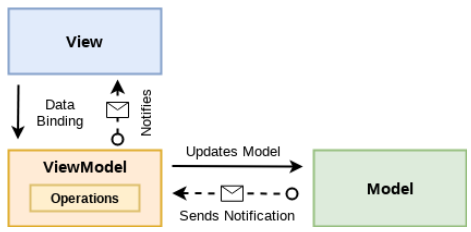
\includegraphics[width=300px]{capitulo5/android/img/capa-presentacion.png}
    \caption{Capa de presentación \cite{cleanWayReload}}
    \label{fig:capa-presentacion}
\end{figure}

En esta capa se pueden trabajar con patrones como MVC y MVP pero en este caso se utiliza el patrón MVVM cada uno con una función en particular. \cite{cleanWayReload}

\begin{itemize}
    \item \textbf{Modelo} Se encarga de representar la información que sera presentada en la vista.
    \item \textbf{Vista} Compuesta en este caso por las actividades y fragmentos de la aplicación, su tarea es mostrar la información, hacen uso de los viewmodels para poder realizar cambios en la interfaz.
    \item \textbf{ViewModel} El ViewModel sera el encargado de ejecutar los casos de uso o interactors con el objetivo de actualizar la vista de acuerdo a la información que presente el modelo.
\end{itemize}



\newpage
\section{Aplicación Web}
\section{Android}
Esta sección tiene objetivo presentar las principales características en el desarrollo de la aplicación para Android.
\subsection{Arquitectura de la aplicación}
Para el desarrollo de la aplicación se implemento la arquitectura Clean, la cual como ya se ha mencionado antes se ha mencionado se ha vuelto muy popular en el desarrollo de aplicaciones móviles para android debido a que es una solución que produce sistemas que presentan las siguientes características.

\begin{itemize}
    \item Escalables, por lo que se pueden agregar más funcionalidades de forma sencilla.
    \item Presentan modularidad.
    \item Presentan independencia en cuanto a frameworks, interfaz de usuario y bases de datos.
    \item El proyecto es más fácil de mantener por lo que es más sencillo hacer cambios.
\end{itemize}

Al utilizar esta arquitectura el proyecto queda separado en tres capas como se observa en la figura \ref{fig:capas-arquitectura} con lo cual cada una de ellas tiene su propósito definido.

\begin{figure}[h]
    \centering
    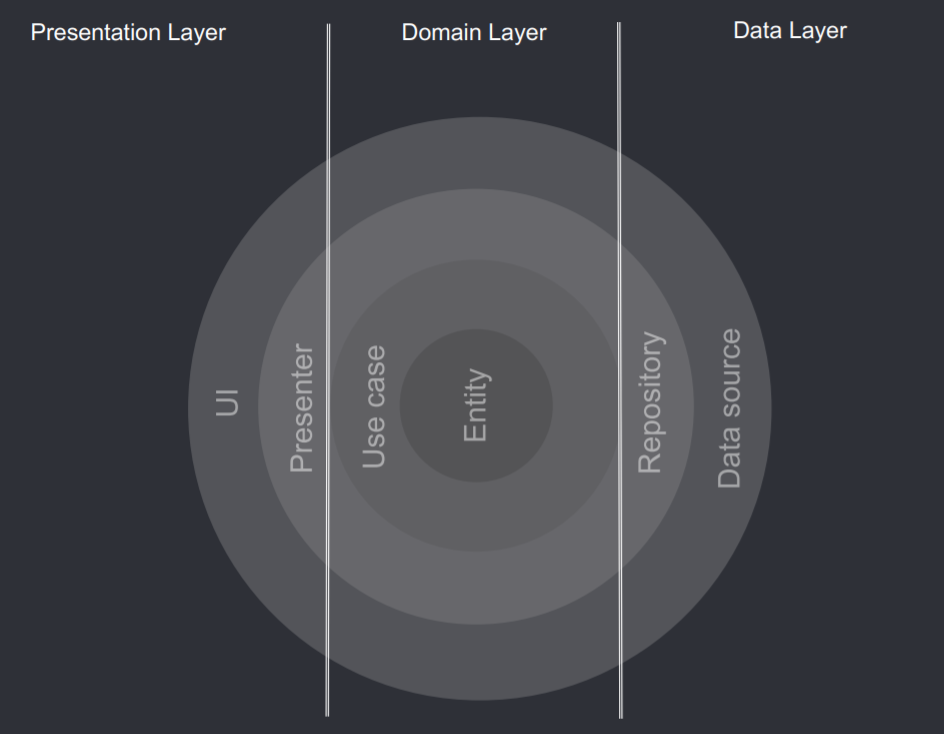
\includegraphics[width=250px]{capitulo5/android/img/capas-clean.png}
    \caption{Tres capas que se tienen al utilizar la arquitectura Clean \cite{cleanGuide}}
    \label{fig:capas-arquitectura}
\end{figure}

\subsubsection{Capa de datos}
La información que se utiliza en el resto de capas proviene de esta capa. Esta capa a su vez se encuentra dividida en la capa de repositorio y en la capa de fuente de datos. 

\paragraph{Capa de repositorio} En esta capa se utiliza el patrón de repositorio como se muestra en la figura \ref{fig:capa-datos}. Gracias a este patrón se puede tener acceso a diferentes fuentes de datos que se encuentran en la capa más baja de nuestra arquitectura, esto nos permite un acceso a los datos de forma transparente para el usuario bajo las condiciones que se presenten.

La forma de utilizar este patrón en la aplicación desarrollado crear una clase en la cual se hace uso de la interfaz que se tiene para el acceso a la fuente de datos. En el siguiente código se puede apreciar el como se crea una instancia de APIService que es nuestra interfaz para fuente de datos.

Después, en nuestro método findAllProyecttosByUser se recupera la información necesaria para mandarla a las capas superiores.

\lstinputlisting[language=Java]{capitulo5/android/src/repositorio.java}

\begin{figure}[h]
    \centering
    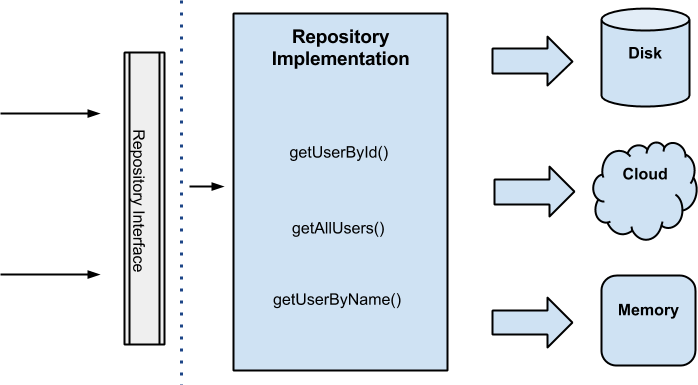
\includegraphics[width=400px]{capitulo5/android/img/capa-datos.png}
    \caption{Capa de datos \cite{cleanWay}}
    \label{fig:capa-datos}
\end{figure}

\paragraph{Capa de fuente de datos} En este trabajo, la fuente de datos que se tiene es un API REST, sin embargo si se requiere acceder a información que se persista en el teléfono se pude agregar otra fuente de datos. Se utilizó retrofit para poder realizar la comunicación con el API REST. 

La forma de utilizar retrofit es crear una interfaz con todos los métodos para recuperar o enviar información al API REST, en esta interfaz cada método tiene la URL a la cual se realizara la petición con alguno de los métodos que tiene HTTP, se tienen los parámetro que se envían y cada método nos regresa una llamada asíncrona que se trabaja en la capa de repositorio. Esto se puede apreciar en el siguiente código.

\lstinputlisting[language=Java]{capitulo5/android/src/APIService.java}

Para poder hacer uso de esta interfaz se tiene que configurar bajo ciertas características especificas como lo son la URL a la cual hará peticiones, el logger que se utilizara para poder observar las peticiones que se realizan y brindar una retroalimentación a la hora de hacer pruebas y por ultimo el parser que se utilizara para trabajar y pasar de clases a datos que el API REST entienda y pueda utilizar, en este caso se utilizo el formato JSON. La definición de estas características se tiene en el siguiente código.

\lstinputlisting[language=Java]{capitulo5/android/src/ServiceGenerator.java}

Finalmente, en esta capa se tienen clases Java que después se mapean a objetos JSON y viceversa, para realizar esto se crea un POJO con los atributos que se necesitan además de agregar anotaciones de retrofit para que el parser pude hacer la conversión necesaria. Un ejemplo de esto es en la siguiente clase de java.

\lstinputlisting[language=Java]{capitulo5/android/src/UsuarioData.java}


\subsubsection{Capa de dominio}
En esta capa es la intermediaria entre las otras dos capas que se tienen, es donde se encuentran los casos de uso también conocidos como interactors como se muestra en la figura \ref{fig:capa-dominio} en ellos la lógica del negocio es ejecutada es por esto que es el núcleo de la aplicación.

Es importante mencionar que esta capa, al ser la encargada del negocio es donde se hacen validaciones en la información y dicha información se adapta para que sea trabajada en la capa de presentación o en la de datos

Además de contener los casos de uso en esta capa se encuentran las entidades y se hace uso de los repositorios para acceder a la información proporcionada por la capa de datos.

\begin{figure}[h]
    \centering
    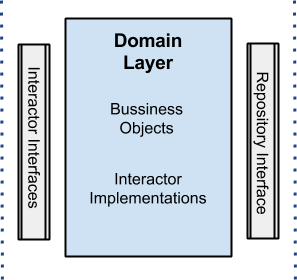
\includegraphics[width=200px]{capitulo5/android/img/capa-dominio.png}
    \caption{Capa de dominio \cite{cleanWay}}
    \label{fig:capa-dominio}
\end{figure}

Para tener un control sobre posibles errores en la capa de presentación o en la capa de datos se utilizan códigos de resultados al igual que una clase que contiene el resultado que se puede presentar, así como la información que se le regresa a la capa de presentación. Se hace uso de genéricos para poder reutilizar esta clase en toda la aplicación y no duplicar código. La clase es la siguiente.

\lstinputlisting[language=Java]{capitulo5/android/src/BusinessResult.java}

La forma en la que se utiliza esta clase en un caso de uso se presenta en el siguiente código que permite iniciar sesión.

\lstinputlisting[language=Java]{capitulo5/android/src/UserInteractorImpl.java}

A su vez el caso de uso utiliza sus propios clases de java para presentar información al usuario en la capa de presentación así como controlar posibles errores en la información que ingrese el usuario los campos de los formularios, un ejemplo de este tipo de clases es el siguiente.

\lstinputlisting[language=Java]{capitulo5/android/src/UsuarioModel.java}

\subsubsection{Capa de presentación}
En esta capa como se muestra en la figura \ref{fig:capa-presentacion} se trabaja con la lógica relacionada a las interfaces que se tienen en la aplicación, es decir a actividades, fragmentos y archivos XML.

\begin{figure}[h]
    \centering
    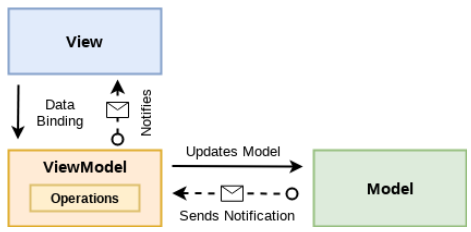
\includegraphics[width=300px]{capitulo5/android/img/capa-presentacion.png}
    \caption{Capa de presentación \cite{cleanWayReload}}
    \label{fig:capa-presentacion}
\end{figure}

En esta capa se pueden trabajar con patrones como MVC y MVP pero en este caso se utiliza el patrón MVVM cada uno con una función en particular. \cite{cleanWayReload}

\begin{itemize}
    \item \textbf{Modelo} Se encarga de representar la información que sera presentada en la vista.
    \item \textbf{Vista} Compuesta en este caso por las actividades y fragmentos de la aplicación, su tarea es mostrar la información, hacen uso de los viewmodels para poder realizar cambios en la interfaz.
    \item \textbf{ViewModel} El ViewModel sera el encargado de ejecutar los casos de uso o interactors con el objetivo de actualizar la vista de acuerdo a la información que presente el modelo.
\end{itemize}



\newpage
\section{Mensajes}
En esta sección se muestran los mensajes que se despliegan en pantalla para los diferentes casos de uso que se tienen.
\begin{enumerate}[label=MSG\arabic*.]
    \item \label{MSG1}
        \begin{description}
            \item \textbf{MSG1 Datos no validos}
            \item [Tipo] Error
            \item [Redacción] Los datos introducidos no son validos.
            %\item [Parametros]
             %\item [Ejemplo]
        \end{description}
    \item \label{MSG2}
        \begin{description}
            \item \textbf{MSG2 Cuenta no verificada}
            \item [Tipo] Error
            \item [Redacción] La cuenta aun no ha sido verificada.
        \end{description}
    \item \label{MSG3}
        \begin{description}
            \item \textbf{MSG3 Correo electrónico no registrado}
            \item [Tipo] Error
            \item [Redacción] No existe una cuenta con el correo electrónico introducido.
        \end{description}
    \item \label{MSG4}
        \begin{description}
            \item \textbf{MSG4 Correo electrónico ya registrado}
            \item [Tipo] Error
            \item [Redacción] El correo electrónico ya se ha utilizado.
        \end{description}
    \item \label{MSG5}
        \begin{description}
            \item \textbf{MSG5 Verifique su cuenta}
            \item [Tipo] Informativo
            \item [Redacción] Verifique su cuenta a través del correo electrónico que se le ha mandado.
        \end{description}
    \item \label{MSG6}
        \begin{description}
            \item \textbf{MSG6 Envio de correo de recuperación}
            \item [Tipo] Informativo
            \item [Redacción] Se ha enviado un correo electrónico para la recuperación de su contraseña.
        \end{description}
    \item \label{MSG7}
        \begin{description}
            \item \textbf{MSG7 No existen proyectos para mostrar}
            \item [Tipo] Informativo
            \item [Redacción] No hay proyectos que se puedan mostrar.
        \end{description}
    \item \label{MSG8}
        \begin{description}
            \item \textbf{MSG8 No se puede mostrar el proyecto}
            \item [Tipo] Error
            \item [Redacción] En este momento no se puede mostrar el proyecto.
        \end{description}
    \item \label{MSG9}
        \begin{description}
            \item \textbf{MSG9 Operación exitosa}
            \item [Tipo] Informativo
            \item [Redacción] La operación se ha realizado con éxito.
        \end{description}
    \item \label{MSG10}
        \begin{description}
            \item \textbf{MSG10 Operación fallida}
            \item [Tipo] Error
            \item [Redacción] La operación no se pudo realizar.
        \end{description}
    \item \label{MSG11}
        \begin{description}
            \item \textbf{MSG11 Confirmación de operación}
            \item [Tipo] Confirmación
            \item [Redacción] \hfill \\
            ¿Está seguro de $<$OPERACIÓN$>$ $<$ELEMENTO$>$ $<$NOMBRE\textunderscore ELEMENTO$>$?
            \item [Parametros] \hfill
                \begin{itemize} 
                    \item $<$OPERACIÓN$>$: Operación a realizar que se debe de confirmar.
                    \item $<$ELEMENTO$>$: Elemento sobre el cual se realizara la operación.
                    \item $<$NOMBRE\textunderscore ELEMENTO$>$: Nombre del elemento sobre el que se trabaja.
                \end{itemize}
            \item [Ejemplo] \hfill
                \begin{itemize}
                    \item ¿Está seguro de eliminar el proyecto tesis final?
                \end{itemize}
        \end{description}
    \item \label{MSG12}
        \begin{description}
            \item \textbf{MSG12 Ingrese el nombre}
            \item [Tipo] Confirmación
            \item [Redacción] Ingrese el nombre del proyecto.
        \end{description}
    \item \label{MSG13}
        \begin{description}
            \item \textbf{MSG13 Falta información}
            \item [Tipo] Error
            \item [Redacción] Falta información necesaria para realizar la operación.
        \end{description}
\end{enumerate}

\newpage
\section{Interfaces}
\subsection{Aplicación en Android}
\begin{figure}[h]
    \centering
    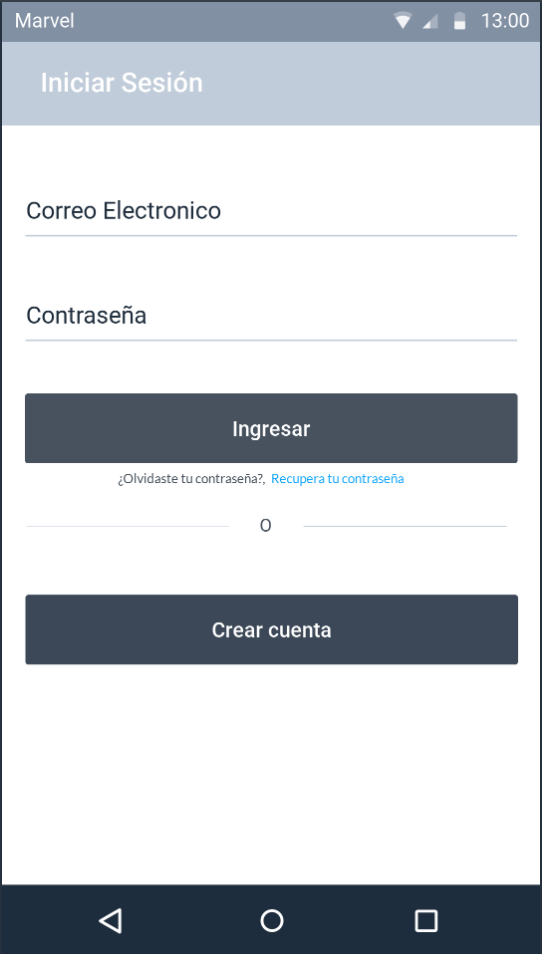
\includegraphics[width=200px]{capitulo4/imagenes/android/MIUA_1.png}
    \caption{MIUA 1 Iniciar Sesión}
    \label{fig:MIUA-1} %MOCK UP DE INTERFAZ DE USUARIO ANDROID
\end{figure}

\begin{figure}[h]
    \centering
    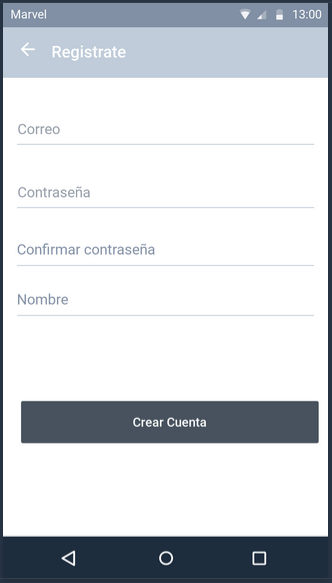
\includegraphics[width=200px]{capitulo4/imagenes/android/MIUA_2.png}
    \caption{MIUA 2 Registro}
    \label{fig:MIUA-2} %MOCK UP DE INTERFAZ DE USUARIO ANDROID
\end{figure}

\begin{figure}[h]
    \centering
    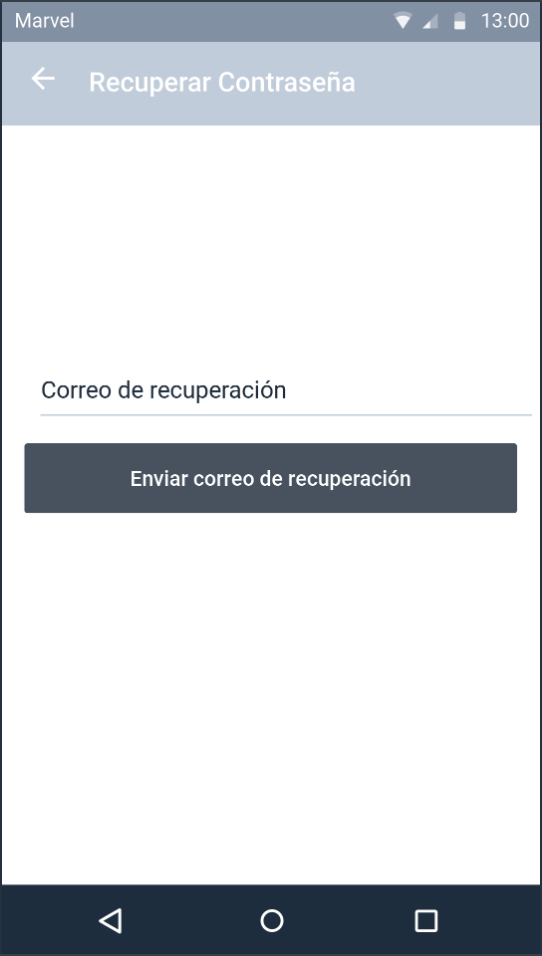
\includegraphics[width=200px]{capitulo4/imagenes/android/MIUA_3.png}
    \caption{MIUA 3 Recuperar Contraseña}
    \label{fig:MIUA-3} %MOCK UP DE INTERFAZ DE USUARIO ANDROID
\end{figure}

\begin{figure}[h]
    \centering
    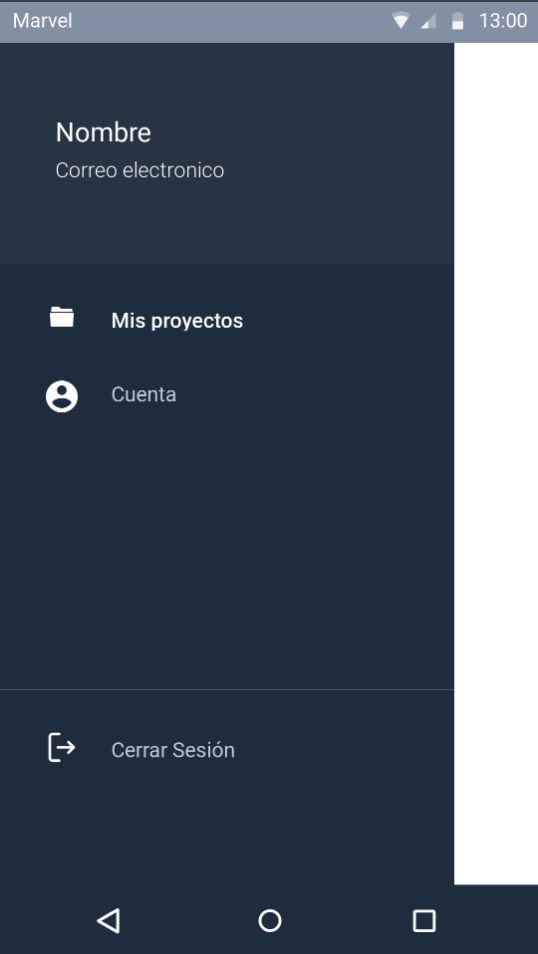
\includegraphics[width=200px]{capitulo4/imagenes/android/MIUA_4.png}
    \caption{MIUA 4 Menú de Opciones}
    \label{fig:MIUA-4} %MOCK UP DE INTERFAZ DE USUARIO ANDROID
\end{figure}

\begin{figure}[h]
    \centering
    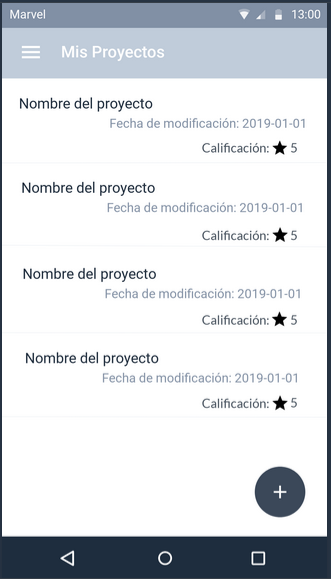
\includegraphics[width=200px]{capitulo4/imagenes/android/MIUA_5.png}
    \caption{MIUA 5 Lista de Proyectos}
    \label{fig:MIUA-5} %MOCK UP DE INTERFAZ DE USUARIO ANDROID
\end{figure}

\begin{figure}[H]
    \centering
    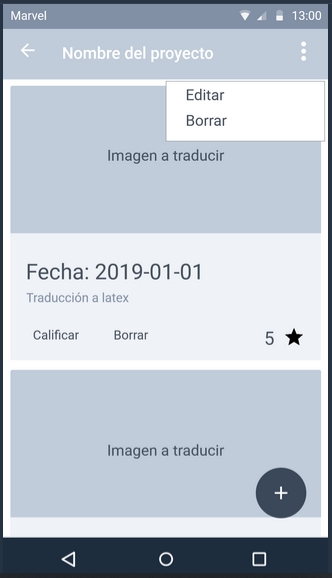
\includegraphics[width=200px]{capitulo4/imagenes/android/MIUA_6.png}
    \caption{MIUA 6 Lista de Traducciones}
    \label{fig:MIUA-6} %MOCK UP DE INTERFAZ DE USUARIO ANDROID
\end{figure}

\begin{figure}[H]
    \centering
    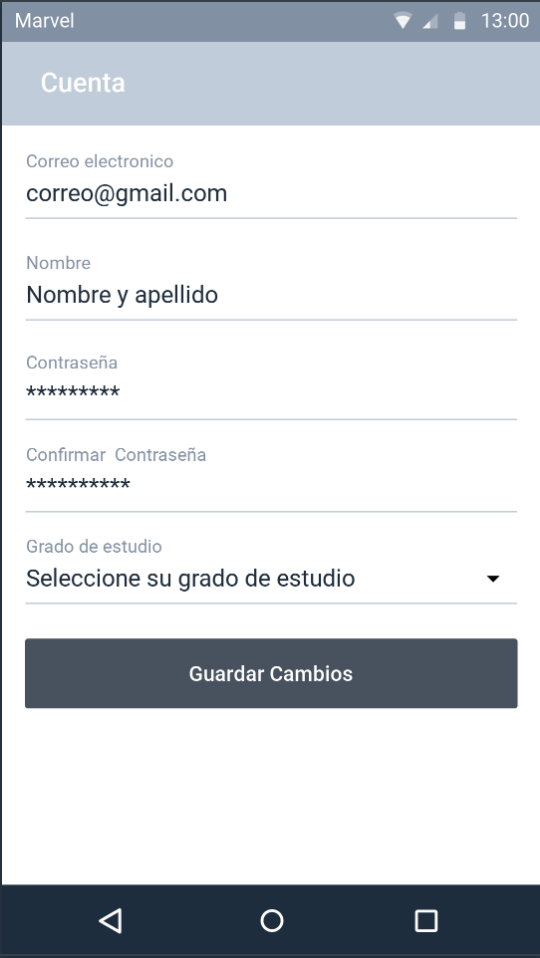
\includegraphics[width=200px]{capitulo4/imagenes/android/MIUA_7.png}
    \caption{MIUA 7 Editar Perfil}
    \label{fig:MIUA-7} %MOCK UP DE INTERFAZ DE USUARIO ANDROID
\end{figure}

\newpage
\subsection{Aplicación en Web}
\begin{figure}[H]
    \centering
    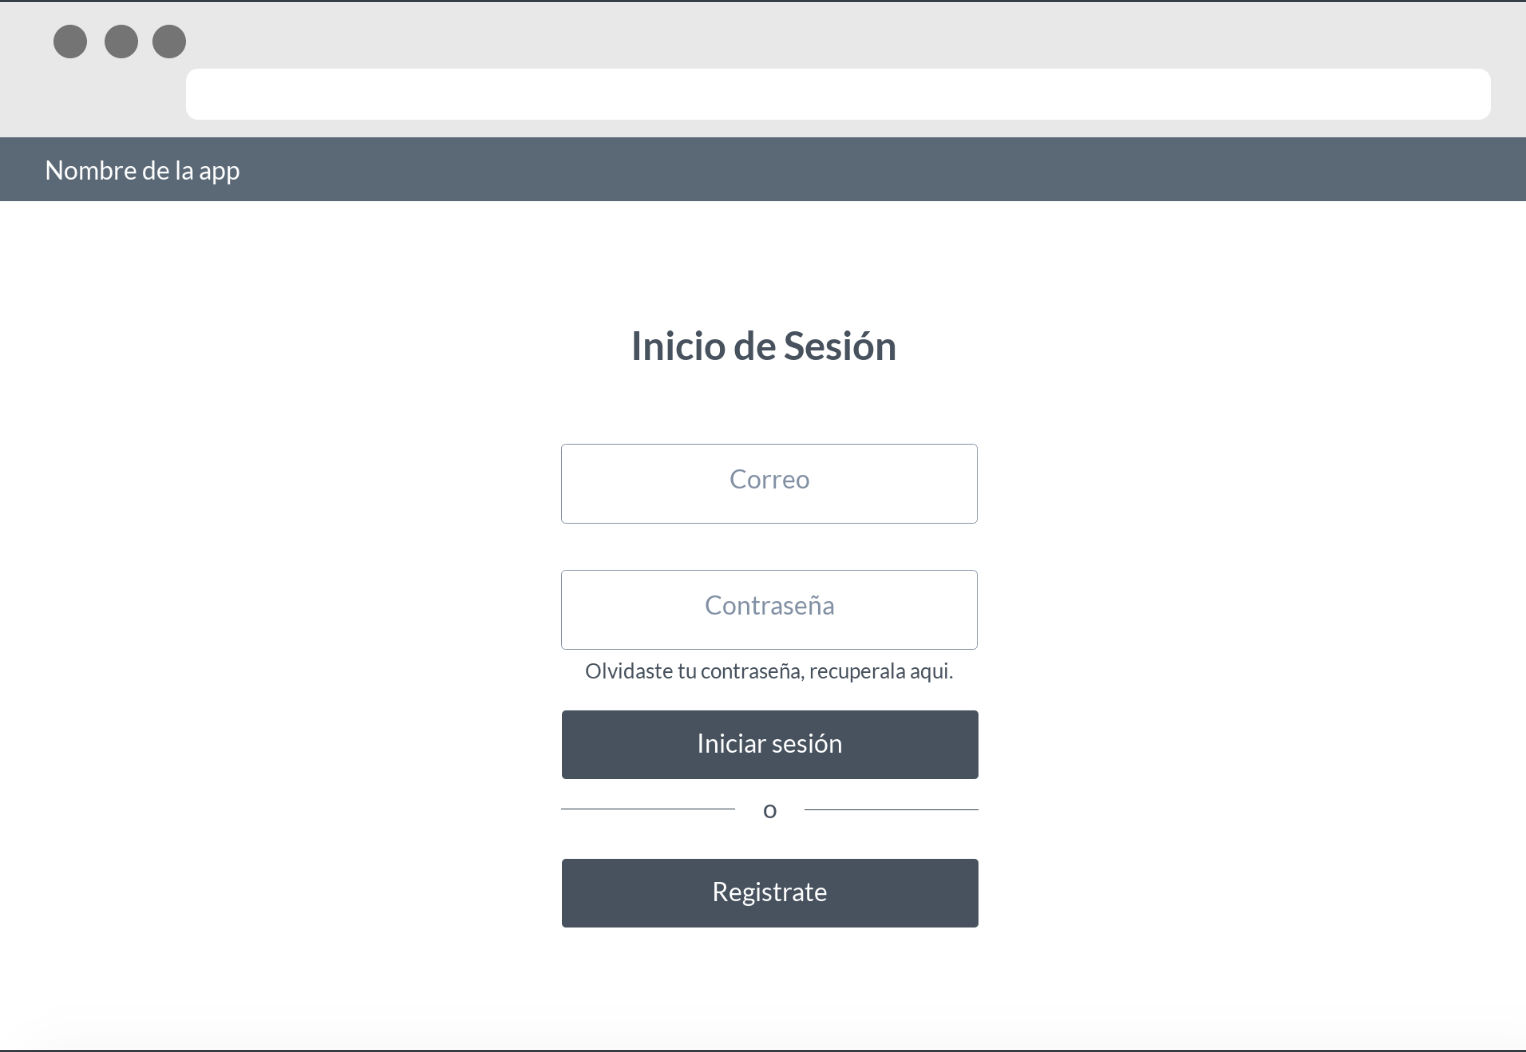
\includegraphics[width=300px]{capitulo4/imagenes/web/IUW_1.png}
    \caption{MIUW 1 Iniciar Sesión}
    \label{fig:MIUW-1}
\end{figure}

\begin{figure}[H]
    \centering
    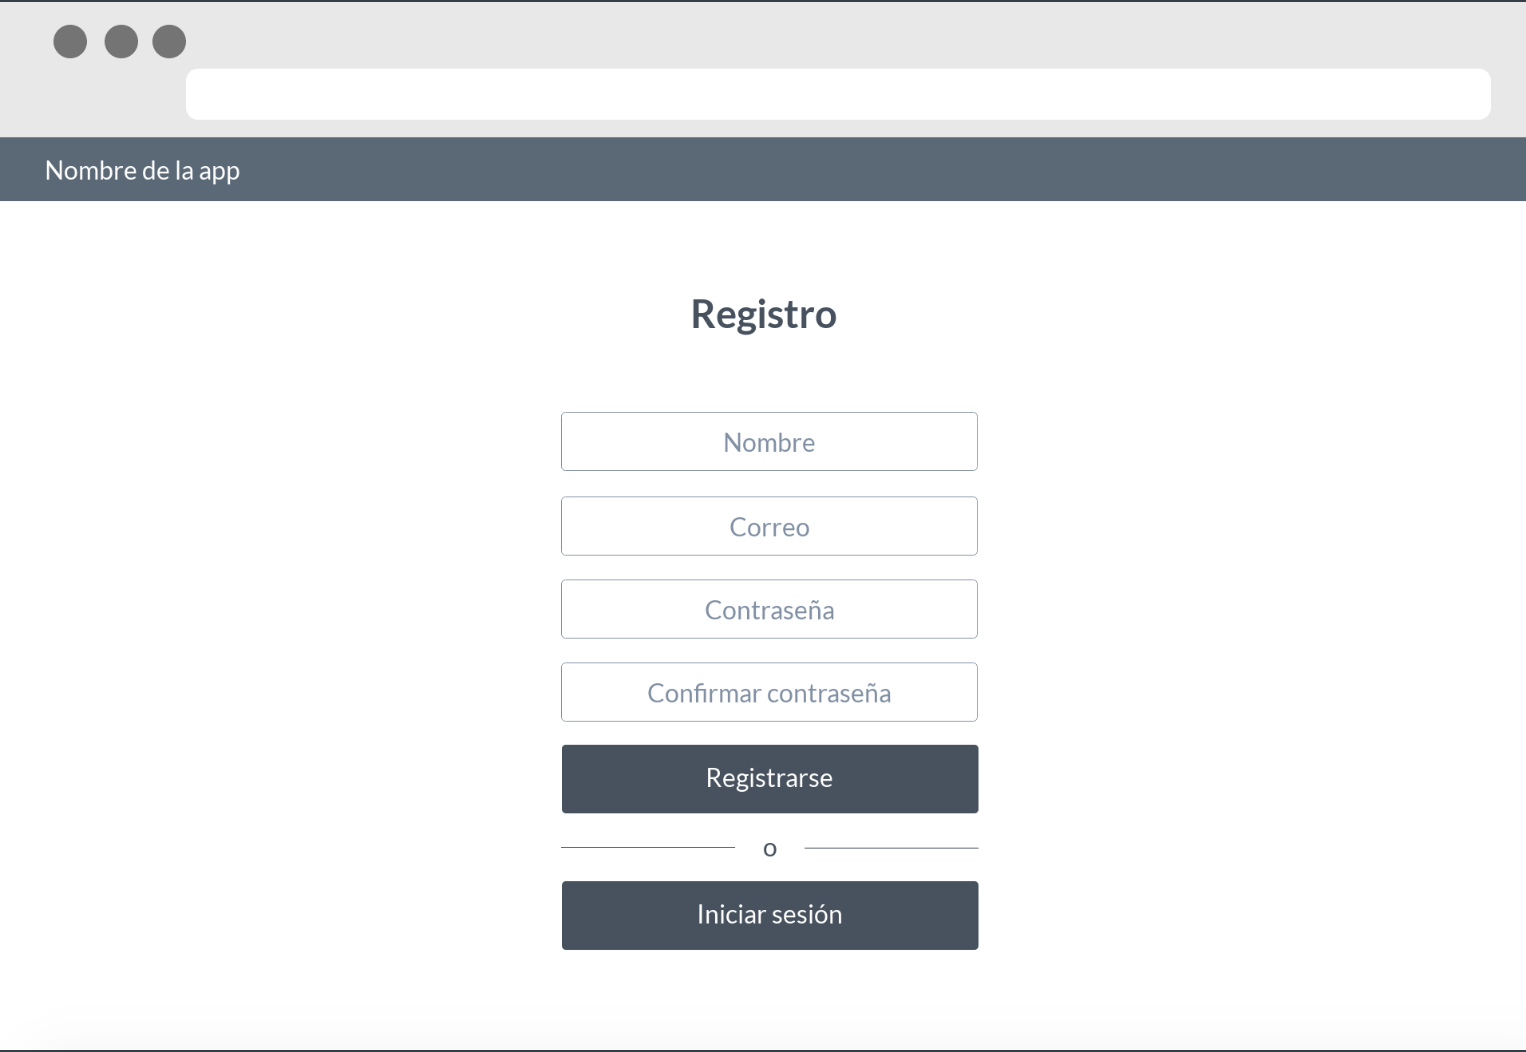
\includegraphics[width=300px]{capitulo4/imagenes/web/IUW_2.png}
    \caption{MIUW 2 Registro}
    \label{fig:MIUW-2}
\end{figure}

\begin{figure}[H]
    \centering
    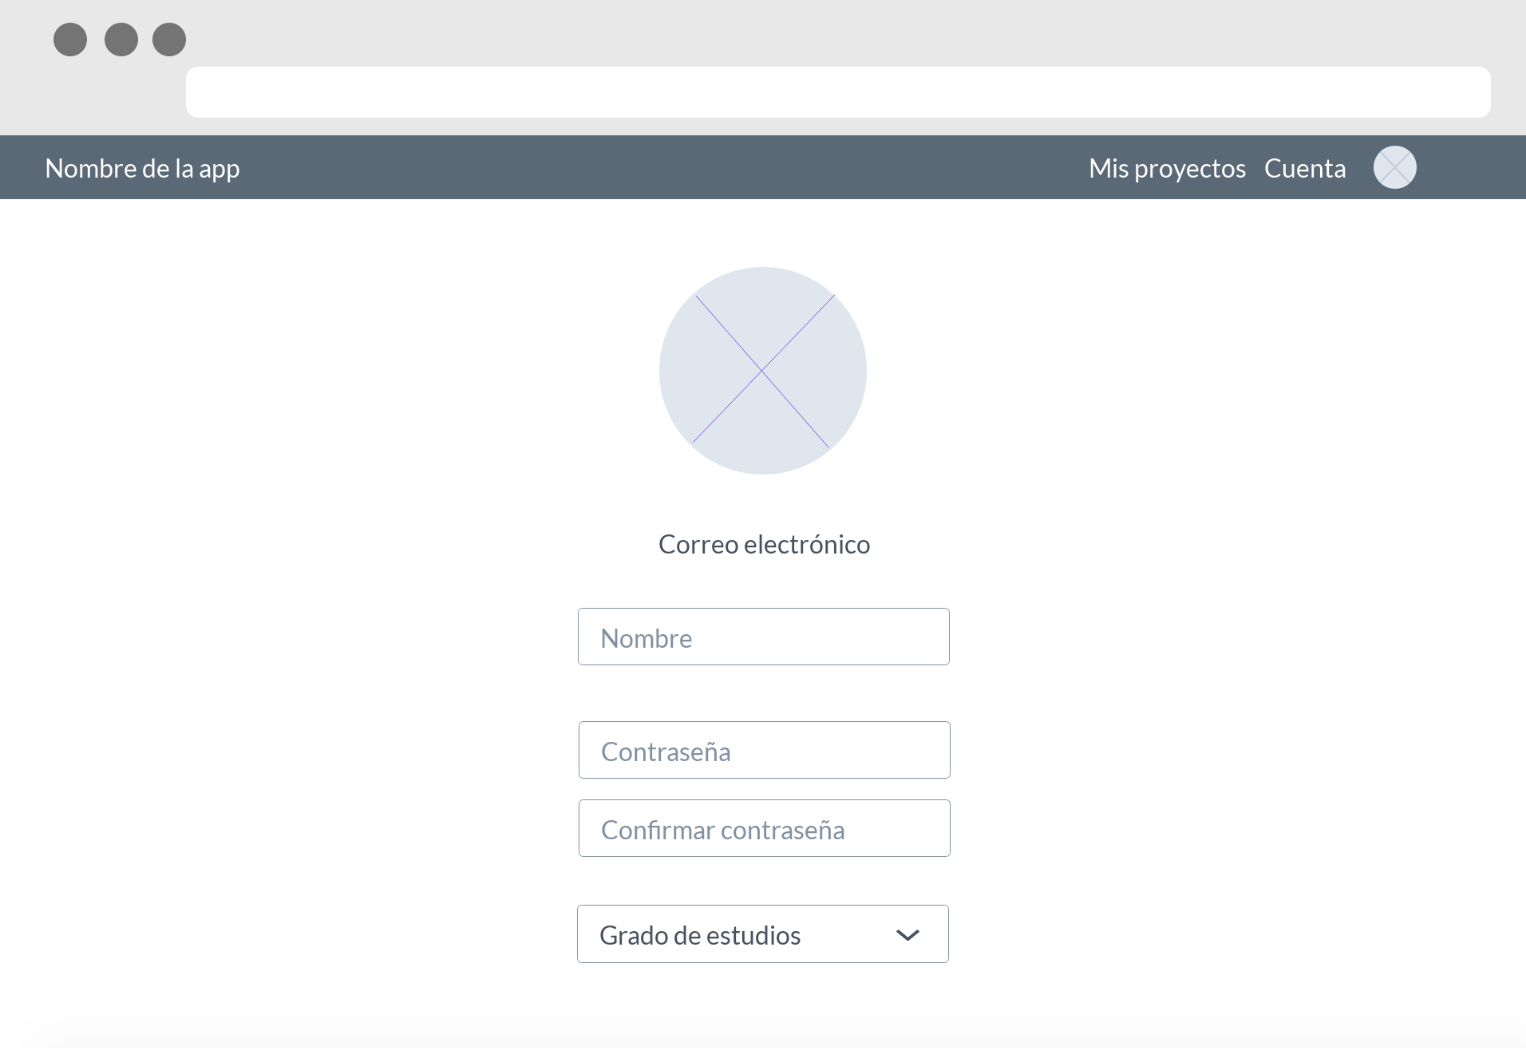
\includegraphics[width=300px]{capitulo4/imagenes/web/IUW_3.png}
    \caption{MIUW 3 Editar Perfil}
    \label{fig:MIUW-3}
\end{figure}

\begin{figure}[H]
    \centering
    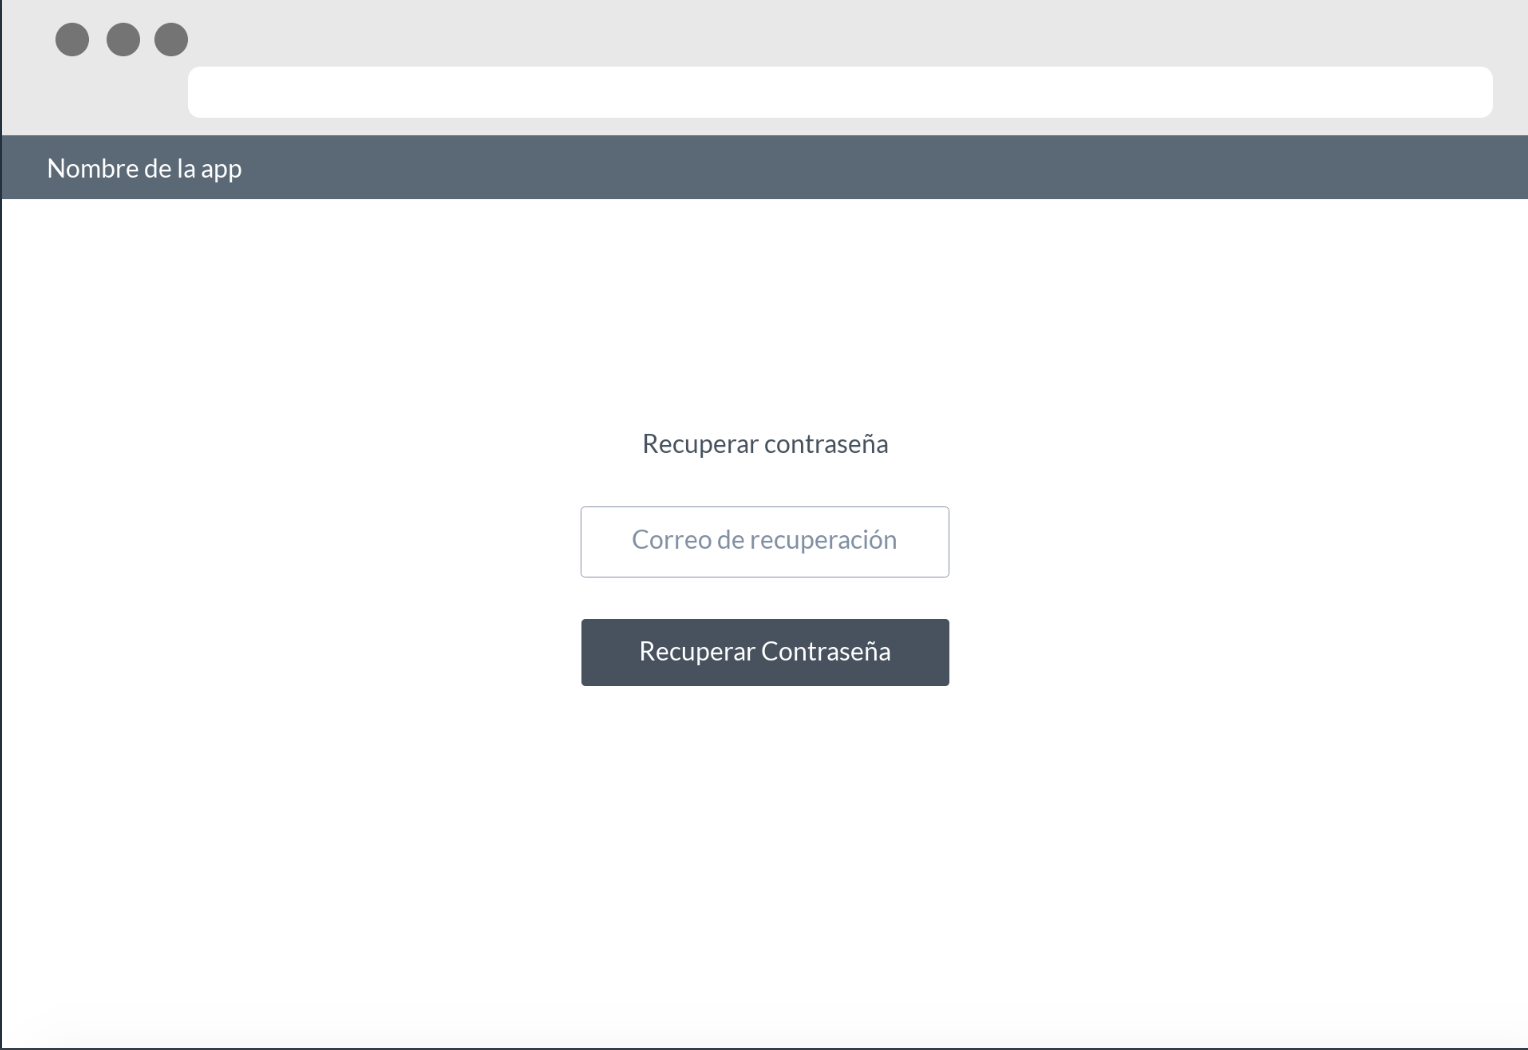
\includegraphics[width=300px]{capitulo4/imagenes/web/IUW_4.png}
    \caption{MIUW 4 Recuperar Contraseña}
    \label{fig:MIUW-4}
\end{figure}

\begin{figure}[H]
    \centering
    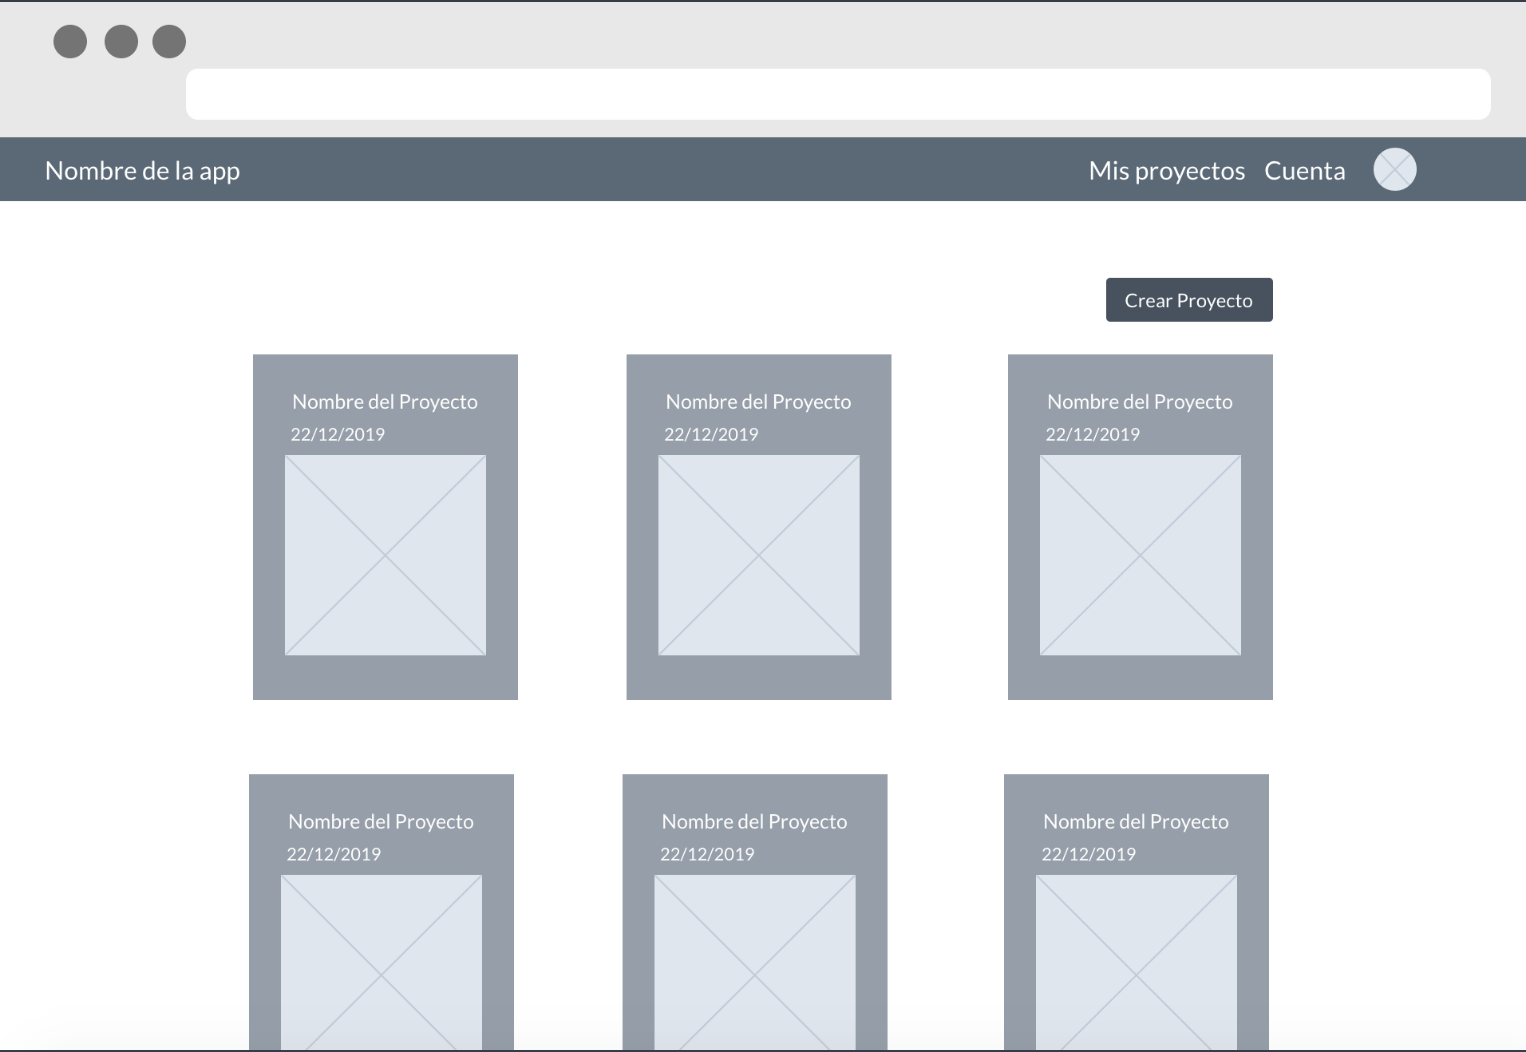
\includegraphics[width=300px]{capitulo4/imagenes/web/IUW_5.png}
    \caption{MIUW 5 Lista de Proyectos}
    \label{fig:MIUW-5}
\end{figure}

\begin{figure}[H]
    \centering
    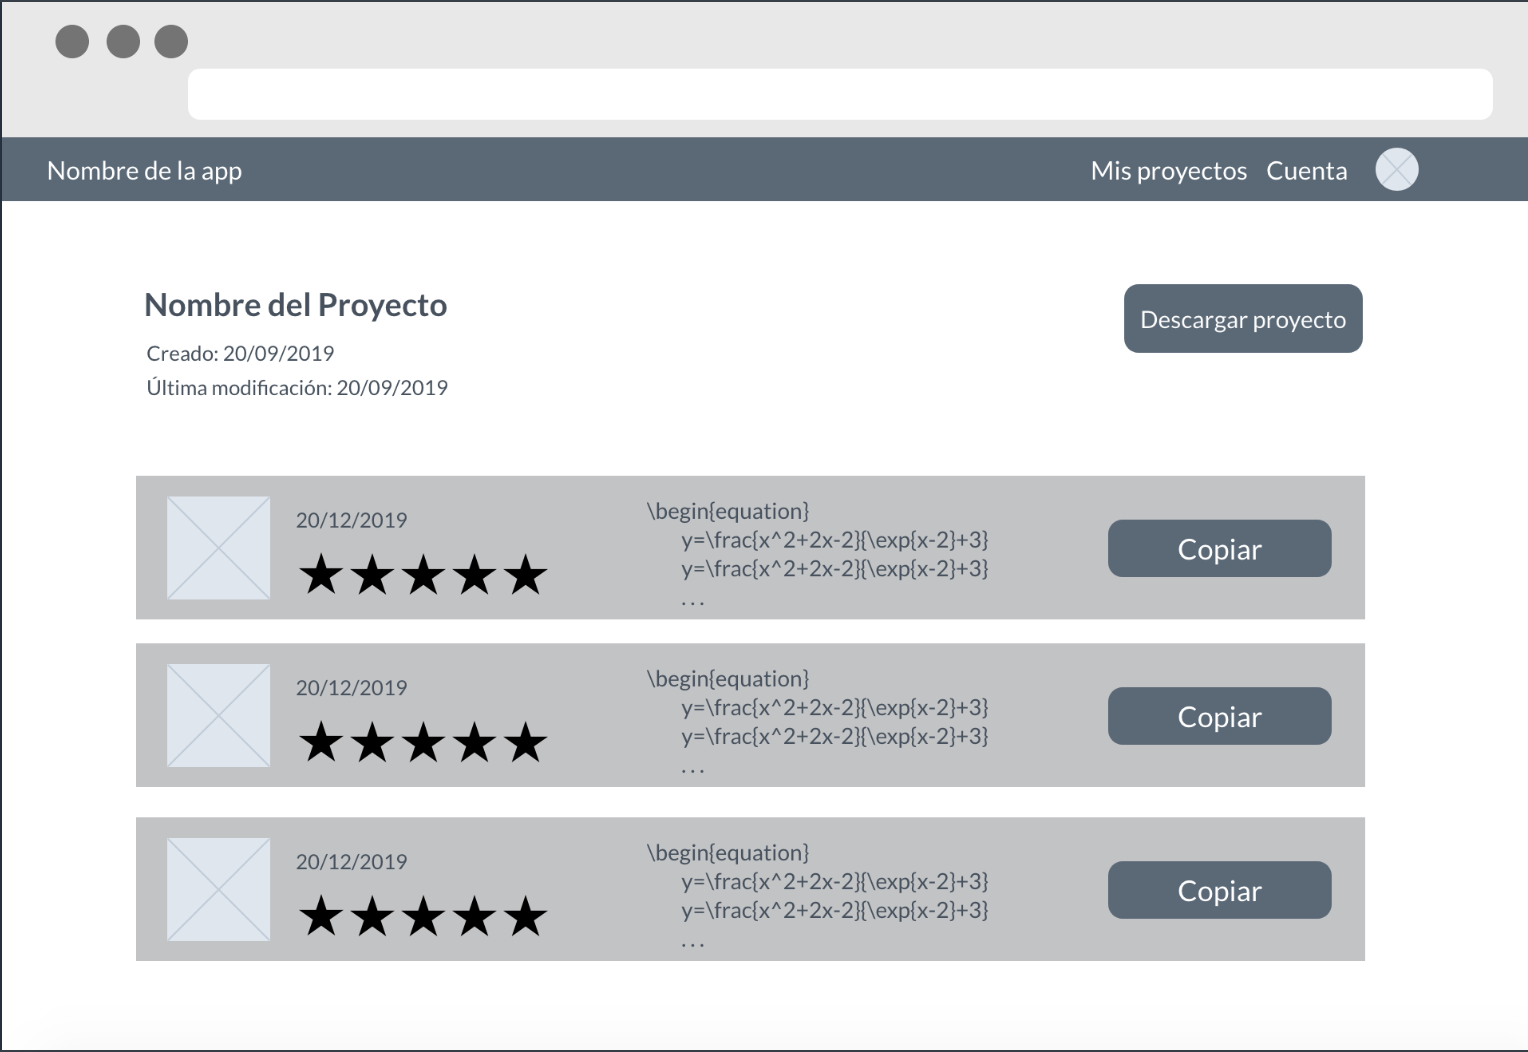
\includegraphics[width=300px]{capitulo4/imagenes/web/IUW_6.png}
    \caption{MIUW 6 Lista de Traducciones}
    \label{fig:MIUW-6}
\end{figure}

\begin{figure}[H]
    \centering
    
\includegraphics[width=300px]{capitulo4/imagenes/web/IUW_7.png}
    \caption{MIUW 7 Menú de Opciones}
    \label{fig:MIUW-7}
\end{figure}
